\documentclass[12pt,oneside,a4paper]{book} % This style for A4 format.

%Packages
\usepackage{ecproject}
\usepackage{graphicx}
\usepackage{tikz}
\usetikzlibrary{calc}
\usepackage[a4paper, margin=1in]{geometry}
\usepackage{float}
\usepackage{qrcode}
%%%Page related
\usepackage{fancyhdr} % for header & footer
\usepackage[hidelinks]{hyperref}
\usepackage[toc, nonumberlist]{glossaries} %For Glossaries - to be loaded only after hyperref package
% For code snippets
\usepackage[listings]{tcolorbox}
    \tcbuselibrary{skins,breakable}
    \tcbuselibrary{theorems}
%\ifIndentPara
\usepackage{indentfirst}
%\fi
\usepackage{setspace}
%%%Table Related
%\usepackage{booktabs}
%\usepackage{makecell}
%\usepackage{multirow}
%\usepackage{multicol}


%Document settings
\title{Design and Implememntation of Beamforming on FPGA}
%%%%%%%%%%%%%%%Minor (or) Major report%%%%%%%%%%%%%%%
%Uncomment \MinorProject line, if the report is for Minor project.
\MinorProject
%%%%%%%%%%%%%%%%%%%%%%%%%%%%%%%%%%%%%%%%%%%%%%
%%%Student Details%%%
\stuNameA{Divam Trivedi}
\stuUSNA{1RV20EC059}
\stuNameB{Jayanthi Abhilash Preetham}
\stuUSNB{1RV20EC080}
%\stuNameC{Subrahmanya K N}
%\stuUSNC{1RV16EC007}
%\stuNameD{Subrahmanya K N}
%\stuUSND{1RV16EC007}

%%%Internal Guide%%%%
\guideNameA{Dr. Nethravathi K. A. }
\guideDesignationA{Assistant Professor}
\guideDeptA{Dept. of ECE}
\guideOrgA{RV College of Engineering}

%%%External Guide%%%%
%\guideNameB{Dr. Usha Rani K. R.}
%\guideDesignationB{Professor}
%\guideDeptB{Dept. of ECE}
%\guideOrgB{RV College of Engineering}

%\guideNameC{Dr. Ramavenkateshwaran}
%\guideDesignationC{Assistant Professor}
%\guideDeptC{Dept. of ECE}
%\guideOrgC{RV College of Engineering}

\panelMemberA{Dr. Usha Rani K. R.}
\panelMemberDesigA{Professor}
\panelMemberB{Dr. Nethravathi K. A.}
\panelMemberDesigB{Assistant Professor}

\Department[ECE]{Electronics and Communication Engineering}

\HOD{Dr. H. V. Ravish Aradhya}
\Principal{Dr. K. N. Subramanya}

\academicYear{2022-23}

\QRurl{}
%\QRurl{https://drive.google.com/open?id=1jm-POmuq-ZZ1tT5m-xAdCDRnwvLZH8q-}
%%%%%%%%%%%%%%%%%%%For PG program%%%%%%%%%%%%%%%%%%%
%%%Uncomment \pgProgram command and define appropriate values for \MastersIn{} and \pgProgramName{}

%\pgProgram%
\MastersIn[B.E.]{Bachelor of Engineering}
\pgProgramName{Electronics \& Communication Engineering}

%%%%%%%%%%%%%%%%%%Draft report%%%%%%%%%%%%%%%%%%
\DraftCopy
%%%%%%%%%%%%%%%%%%%%%%%%%%%%%%%%%%%%%%%%%%%%%%

%%%%%%%%%%%%%%%%%%Acronyms%%%%%%%%%%%%%%%%%%
\newglossary[sym]{symbolList}{sym1}{sym2}{List of Symbols}
\makeglossaries
%Acronyms
\loadglsentries{./AuxFiles/Glossaries}
\renewcommand{\glspostdescription}{}% To remove dot at the end
%%%%%%%%%%%%%%%%%%%%%%%%%%%%%%%%%%%%%%%%%%%%%%

%%%%%%%%%%%%%%Bibliography%%%%%%%%%%%%%%%%%%%%%
\usepackage[backend=bibtex,style=ieee]{biblatex}
%If backend is set to bibtex, then configure texmaker Bi(La)Tex with "bibtex %"
\addbibresource{./AuxFiles/ProjectBib.bib}%Add bib file with extention
%%%%%%%%%%%%%%%%%%%%%%%%%%%%%%%%%%%%%%%%%%%%%%

%%%%%%%%%%%%%%%%WaterMark%%%%%%%%%%%%%%%%%%%%%
%%Use it only after Biblatex
%\usepackage[printwatermark]{xwatermark}
%\newwatermark[allpages,color=gray!50,angle=0,scale=2,xpos=0,ypos=0]{
\includegraphics[width=0.3\textwidth]{Figures/RVlogoVecW}}
%\usepackage{background}
%\backgroundsetup{scale=1, angle=0, firstpage = true, opacity=1, contents={
%\begin{tikzpicture}[remember picture, overlay]
%\node at ([yshift=0pt, xshift=0pt]current page.center){\includegraphics[width=0.3\textwidth]{Figures/RV_logoVecW}};
%\end{tikzpicture}
%}}
%%%%%%%%%%%%%%%%%%%%%%%%%%%%%%%%%%%%%%%%%%%%%%
\begin{document}
\maketitle
%\pagestyle{empty}
\newpage
\begin{spacing}{1.5}
%%ecproject package is created by P Narashimaraja, Assistant Professor, ECE, RVCE
%Border
\begin{tikzpicture}[remember picture, overlay]
  \draw[line width = 4pt] ($(current page.north west) + (0.75in,-0.75in)$) rectangle ($(current page.south east) + (-0.75in,0.75in)$);
\end{tikzpicture}
\thispagestyle{empty}
\vspace{-1cm}
\begin{center}
\Large\textbf{RV College of Engineering\textsuperscript{\small\textregistered}, Bengaluru} \par
\large{(\textit{Autonomous institution affiliated to VTU, Belagavi})} \par
\large\textbf{Department of \printDepartmentLF}\\
.\hspace{2cm}\\

\includegraphics[width=4cm]{Figures/RV_logoVec}\par
\Large\textbf{\underline{CERTIFICATE}} \par
\end{center}
%\begin{minipage}[b]{\linewidth}
%\large
\begin{spacing}{1.5}
\noindent Certified that the \ifMinor{minor\;}\else{ major\;}\fi project (18EC81)work titled \textbf{\textit{\printTitle}} is carried out by
\ifPG{%
\textbf{\printStuNameA} (\textbf{\printStuUSNA}) who is  bonafide student 
}
\else{
\ifStuNameDUsed{%
\textbf{\printStuNameA } (\textbf{\printStuUSNA}), \textbf{\printStuNameB } (\textbf{\printStuUSNB}), \textbf{\printStuNameC } (\textbf{\printStuUSNC}) and \textbf{\printStuNameD } (\textbf{\printStuUSND})  who are bonafide students 
}\else{% 
\ifStuNameCUsed{%
\textbf{\printStuNameA } (\textbf{\printStuUSNA}), \textbf{\printStuNameB } (\textbf{\printStuUSNB}) and \textbf{\printStuNameC } (\textbf{\printStuUSNC})  who are bonafide students 
}\else{%
\ifStuNameBUsed{%
\textbf{\printStuNameA} (\textbf{\printStuUSNA}) and \textbf{\printStuNameB} (\textbf{\printStuUSNB})  who are bonafide students 
}\else{%
\textbf{\printStuNameA} (\textbf{\printStuUSNA}) who is  bonafide student 
}
\fi
}\fi
}\fi
}\fi
of RV College of Engineering, Bengaluru, in partial fulfillment of the requirements for the degree of  \ifPG \textbf{\printMastersInLF} in \textbf{\printMastersPrgName} \else\textbf{Bachelor of Engineering} in \textbf{\printDepartmentLF} \fi of the Visvesvaraya Technological University, Belagavi during the year \printAcadYear. It is certified that all corrections/suggestions indicated for the Internal Assessment have been incorporated in the \ifMinor{minor\;}\else{major\;}\fi project report deposited in the departmental library. The \ifMinor{minor\;}\else{ major\;}\fi project report has been approved as it satisfies the academic requirements in respect of \ifMinor{minor\;}\else{ major\;}\fi project work prescribed by the institution for the said degree.\\ \par
\end{spacing}

\begin{table}[H]
\centering
\resizebox{1\textwidth}{!}{%
\begin{tabular}{ccc}
\large Signature of Guide &\large Signature of Head of the Department &\large Signature of Principal\\
& &\\
\large\printGuideNameA & \large\printHOD & \large\printPrincipal\\
& & \\
\end{tabular}%
}
\end{table}

\begin{table}[H]
\centering
%\resizebox{\textwidth}{!}{%
\begin{tabular}{lccp{6cm}cc}
&&&\textbf{External Viva}&&\\
&&&&&\\
&Name of Examiners &&& & Signature with Date\\
&&&&&\\
1.&&&&&\\
&&&&&\\
2.&&&&&\\
\end{tabular}%
%}
\end{table}
%\pagebreak

\newpage
%%ecproject package is created by P Narashimaraja, Assistant Professor, ECE, RVCE
%%Border
\begin{tikzpicture}[remember picture, overlay]
  \draw[line width = 4pt] ($(current page.north west) + (0.75in,-0.75in)$) rectangle ($(current page.south east) + (-0.75in,0.75in)$);
\end{tikzpicture}

\thispagestyle{empty}

\begin{center}
\Large\textbf{\underline{DECLARATION}} \par
\end{center}


\noindent \ifPG I \else \ifStuNameBUsed We\else I\fi\fi, \textbf{\printStuNameA} \ifPG \else\ifStuNameBUsed  \ifStuNameCUsed ,$\,$ \else{$\,$ and $\,$}\fi \textbf{\printStuNameB} \ifStuNameCUsed  \ifStuNameDUsed ,$\,$ \else{$\,$ and $\,$}\fi \textbf{\printStuNameC}$\,$ \ifStuNameDUsed and $\,$ \textbf{\printStuNameD}$\,$ \fi \fi \fi \fi students of \ifPG fourth \else \ifMinor{seventh\;}\else{eighth\;}\fi \fi semester \ifPG \printMastersInSF\, in \printMastersPrgName \else B.E.\fi, Department of \printDepartmentLF, RV College of Engineering, Bengaluru, hereby declare that the \ifMinor{minor\;}\else{ major\;}\fi project titled `\textbf{\printTitle}' has been carried out by \ifStuNameBUsed us \else me \fi and submitted in partial fulfilment for the award of degree of \ifPG \textbf{\printMastersInLF} in \textbf{\printMastersPrgName} \else\textbf{Bachelor of Engineering} in \textbf{\printDepartmentLF} \fi during the year \printAcadYear.\\ \par

\noindent Further \ifPG I \else\ifStuNameBUsed we \else I \fi \fi declare that the content of the dissertation has not been submitted previously by anybody for the award of any degree or diploma to any other university.\\ \par

\noindent \ifPG I \else\ifStuNameBUsed We \else I \fi \fi also declare that any Intellectual Property Rights generated out of this project carried out at RVCE will be the property of RV College of Engineering, Bengaluru and we will be one of the authors of the same.

\vspace{1cm}
\noindent Place: Bengaluru\par
\vspace{0.5cm}
\noindent Date: \par

\vspace{2cm}
\begin{table}[H]
\centering
%\resizebox{\textwidth}{!}{%
\begin{tabular}{llcp{5cm}cc}
&&&&&\\
&&&&&\\
&Name  &&& Signature& \\
&&&&&\\
1.&\printStuNameA (\printStuUSNA)&&&&\\
&&&&&\\
\ifPG% 
\else%
\ifStuNameBUsed%
2.&\printStuNameB (\printStuUSNB)&&&&\\
&&&&&\\
\else%
\fi%
\ifStuNameCUsed%
3.&\printStuNameC (\printStuUSNC)&&&&\\
&&&&&\\
\else%
\fi%
\ifStuNameDUsed%
4.&\printStuNameD (\printStuUSND)&&&&\\
&&&&&\\
\else%
\fi%
\fi%
\end{tabular}%
%}
\end{table}
%\pagebreak


\newpage
%%ecproject package is created by P Narashimaraja, Assistant Professor, ECE, RVCE.
%%Border
\begin{tikzpicture}[remember picture, overlay]
  \draw[line width = 4pt] ($(current page.north west) + (0.75in,-0.75in)$) rectangle ($(current page.south east) + (-0.75in,0.75in)$);
\end{tikzpicture}
\thispagestyle{empty}

\begin{center}
%.\hspace{1cm}\\ \par
\Large\textbf{\underline{ACKNOWLEDGEMENT}} \par
\end{center}

\ifPG I am \else
\ifStuNameBUsed We are \else I am \fi\fi indebted to \ifPG my \else\ifStuNameBUsed our \else my \fi\fi guide, \textbf{\printGuideNameA}, \printGuideDesigA, \printGuideOrgA$\,.$ for the wholehearted support, suggestions and invaluable advice throughout \ifPG my \else\ifStuNameBUsed our \else my \fi\fi project work and also helped in the preparation of this thesis.\\ \par

\ifPG I \else \ifStuNameBUsed We \else I \fi\fi also express our gratitude to \ifPG my \else\ifStuNameBUsed our \else my \fi\fi  panel members \textbf{\printPanelMemberA}, \printPanelMemberDesigA $\,$ and \textbf{\printPanelMemberB}, \printPanelMemberDesigB , Department of \printDepartmentLF\, for their valuable comments and suggestions during the phase evaluations. \\ \par

\ifPG My \else \ifStuNameBUsed Our \else My \fi\fi sincere thanks to the project coordinators \textbf{Dr. Nethravathi K. A.} for her timely instructions and support in coordinating the project.\\ \par

\ifPG My \else \ifStuNameBUsed Our \else My \fi\fi gratitude to \textbf{Prof. Narashimaraja P} for the organized latex template which made report writing easy and interesting.\\ \par


\ifPG My \else \ifStuNameBUsed Our \else My \fi\fi sincere thanks to \textbf{\printHOD}, Professor and Head, Department of \printDepartmentLF, RVCE for the support and encouragement.\\ \par

\ifPG I \else \ifStuNameBUsed We \else I \fi\fi express sincere gratitude to our beloved Principal, \textbf{\printPrincipal} for the appreciation towards this project work.\\ \par

\ifPG I \else\ifStuNameBUsed We \else I \fi\fi thank all the teaching staff and technical staff of \printDepartmentLF\, department, RVCE for their help.\\ \par 

Lastly, \ifPG I \else\ifStuNameBUsed we \else I \fi\fi take this opportunity to thank \ifPG my \else\ifStuNameBUsed our \else my \fi\fi family members and friends who provided all the backup support throughout the project work.\\ \par

%\pagebreak
\newpage
\pagenumbering{roman}
\chapter*{Abstract}
\addcontentsline{toc}{chapter}{Abstract}\vspace{-1cm}
%Border
\begin{tikzpicture}[remember picture, overlay]
  \draw[line width = 4pt] ($(current page.north west) + (0.75in,-0.75in)$) rectangle ($(current page.south east) + (-0.75in,0.75in)$);
\end{tikzpicture}


Highlights of significant contributions: One page with 3 to 4 paragraphs\\

Paragraph 1: Importance and relevance of Topic, reported issues and limitations of the topic in performance or computation etc, issues involved in those limitations, need for addressing those issues and a short note on how that is addressed in this report.


Paragraph 2 Objectives of this work, short note on algebraic methods used and formulations achieved, computational procedures developed. \gls{ic}.


Paragraph 3: Description of simulation procedure including SW tools used and choice of test cases. Short note on results achieved and significant highlights of improvements if any in terms of percentage , for example the architecture presented in this report shows 22 \% improve in power consumption as compared to the previously reported articles.
\gls{ic}

Paragraph 4:The last para needed only if emulation (after simulation) or Hardware developed to validate simulation results in para 3. 

\pagebreak
\end{spacing}
\newpage
\pagestyle{fplain}
\begin{spacing}{1.5}
	\tableofcontents	
\end{spacing}
\newpage
\begin{spacing}{1.5}
	\cleardoublepage
	\addcontentsline{toc}{chapter}{\listfigurename}
	\listoffigures	
\end{spacing}
\newpage
\begin{spacing}{1.5}
	\cleardoublepage
	\addcontentsline{toc}{chapter}{\listtablename}
	\listoftables	
\end{spacing}
\newpage
\printglossary[type=\acronymtype, title= Abbreviations, toctitle=Abbreviations]
\newpage
\printglossary[type=symbolList, title= List of Symbols, toctitle=List of Symbols]

\mainmatter
\pagestyle{mplain}
\glsresetall
\begin{spacing}{1.5}
%Chapter 1 
\chapter{Introduction to Beamforming}

\section[Introduction]{\textbf{Introduction}}
In the era of ubiquitous connectivity, wireless communication has become an indispensable aspect of our daily lives. From smartphones to IoT devices, the demand for faster, more reliable, and more efficient wireless networks continues to escalate. To address these challenges, researchers and engineers have turned their attention to beamforming - a transformative technology that revolutionizes wireless communication systems.

\begin{figure}[htb]
\centering
	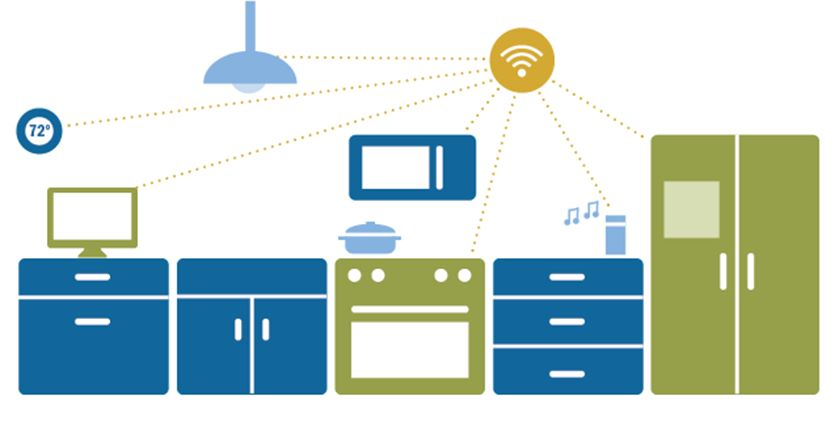
\includegraphics[scale=0.5]{Chapter1/Figures/era}	
	\caption{\label{fig:era}Era of Ubiquitous Connectivity}
\end{figure}

Beamforming is an advanced signal processing technique that enables the focused transmission and reception of electromagnetic waves. By dynamically steering the antenna array's radiation pattern towards specific targets, beamforming offers significant advantages over conventional broadcasting methods. This technology maximizes signal quality, extends coverage range, and enhances network capacity, making it a fundamental area of research and development in the field of wireless communication.

The quest for higher data rates, improved coverage, and enhanced spectral efficiency has led to the emergence of hybrid beamforming techniques. Hybrid beamforming combines the benefits of analog and digital beamforming, offering a promising solution to address the challenges of next-generation wireless networks. To effectively implement hybrid beamforming algorithms, the use of Field-Programmable Gate Arrays (FPGAs) has gained considerable attention due to their flexibility, reconfigurability, and high processing capabilities.

The efficient implementation of hybrid beamforming algorithms necessitates significant computational capabilities, real-time processing, and flexibility to adapt to changing channel conditions. FPGAs provide an ideal platform to address these requirements. Their parallel processing architecture, reconfigurability, and low-latency characteristics make them well-suited for implementing complex digital signal processing tasks, including the extensive matrix operations involved in hybrid beamforming.

\section[Motivation]{\textbf{Motivation}}

As budding engineers of the 21st century, technology is no foreign to us. As a student ourselves, we have at least two if not more smart devices connected to the net at all times. Now with the onset of 5G cellular technology, our expectations wrt data usage has increased even more with ultra fast connectivity becoming a common norm. No doubt our world is progressing in communication technologies and still, we can’t help but wonder why do we still face connection losses while talking on calls! While on a quest to understand the reason behind this, we stumbled upon something called Beamforming and we put our engineering minds to take it upon us and try to improve and explore this major domain of communication engineering! 


\section[Problem statement]{\textbf{Problem statement}}

The design and implementation of a hardware solution for adaptive beamforming pose significant challenges. The problem at hand is to develop a hardware design that effectively adapts to the inbuilt and predefined conditions of the adaptive beamforming, as well as the varying test environments of targets and interferences.

\section[Objectives]{\textbf{Objectives}}
The objectives of the project are
\begin{enumerate}
\item To design and implement a flexible, reconfigurable, and low-latency beamforming algorithm on FPGA.
\item Benchmarking the performance of the implemented design with respect to various parameter constraints such as Speed, Area Utilization and Power consumption and comparing it with the theoretical requirements and other existing beamforming technologies.
\end{enumerate}

\section[Literature Review]{\textbf{Literature Review}}

\textbf{Van Veen et al [1]} classifies beamformers into data independent or statistically optimum, depending on how the weights are chosen. Both are defined with respect to array data where the output of both scenarios are used to optimize the array response. The same procedure is extended to and implemented in spatial filtering.

\textbf{Benesty et al [2]} discusses couple of beamforming techniques by dividing spatial filtering into two parts being synchronization and weight-sum. both methods are discussed with their effects on the beam pattern that is their characteristics of side lobe and main lobe. Beamformers would not yield the same beam pattern for different frequencies and the beam width decreases as the frequency increases.

\textbf{Mucci et al [3]} explains that an input sampling rate Fs, significantly greater than that required for waveform reconstruction, is needed to achieve acceptable approximations to the exact steering delays; frequently, the input sampling rate is five to ten times that required for waveform reconstruction. Interpolation Beamforming  technique is used  for low pass(using zero padding to get higher frequencies) as well as bandpass applications (using Analytic Signal Sampling, Second order Signal Sampling)\\
\textbf{Ulrich et al [7]} explains the need for adaptive array processing in the presence of multiple jammers, conditions for optimal weight computation (SNR), adaptive weight estimation, problems involved in adaptive beamforming,adaptive detection using Maximum Likelihood (ML), Need for Direction of Arrival (DOA)- super resolution.\\
\textbf{Ulrich et al [10]} looks into the grating problem occurring at subarray outputs. s optimization techniques are compared with comparison of resulting grating lobes. The paper concludes that partially overlapping subarrays are the most suited configuration to reduce grating lobes.\\
\textbf{Ulrich et al [11]} defines the advantages of such a design and the analysis. An array containing subarrays is a fairly wide concept that encompasses the situation of steerable directional array elements. At the elements, only phase shifters can also be used to steer all subarrays in a specific direction, and attenuation can be used to control the sidelobe level. The sum of the subarrays then yields the sum beam output. The subarrays may be considered as a super array with components with distinct patterns directed in the desired direction. A completely digital array with Analog to Digital Converters (ADC)s at each antenna element may be ideal, however, it is not practical due to its high weight and cost, resulting in a system with fewer digital receivers.\\
\textbf{Sivasanka et al [5]} explains the effect of the sub array configuration on adaptive beam forming and grating notches in detail with simulation results for ULA. Adaptive beamforming algorithm by using sub arrays, Antenna element and sub-array configurations for simulations has also been shown.\\
\textbf{Zhen-Hai Xu et al [8]} explains how a smart partitioning of a very large planar array into a number of separately fed subarrays offers many interesting design possibilities in antenna synthesis problems. Two typical requirements for the beam scanning - a minimum gain requirement and a sidelobe level requirement - are analyzed whose numerical results illustrate the LFOV technology and validate the analyses.\\
\textbf{Heidelberg et al [1]} decouples Spatial filtering operation into two sub-processes: synchronization and weight-and-sum. The synchronization part controls the steering direction and the weight-and-sum process controls the beamwidth of the main lobe and the characteristics of the sidelobes. Beamformers would not yield the same beam pattern for different frequencies and the beam width decreases as the frequency increases.\\
\textbf{Patel et al [4]} compares Adaptive Beamforming Algorithms LMS, SMI and RLS for ULA Smart Antenna. The radiation pattern achieved by using LMS algorithm is finest. Convergence speed is one the drawback of LMS algorithm as it is directly depends on the step size value. Convergence is low for small value of step size and for large value of step size it becomes unstable. SMI overcomes the limitation of LMS but it increase the complex computation of correlation matrix. RLS algorithm array weights are updates very quickly because the variation of convergence is determined by the knowledge of eigen value of the correlation matrix of signal.\\ 
\textbf{Digdarsini et al [5]} discuss the hardware for digital subsystem consisting of the ADCs, Buffers, FPGA and DAC. The most critical requirement for any DBF system is the reception of the signals from antenna elements at equal phases for baseband processing. This equi-phase clock distribution is achieved by a 1:16 clock distribution card which provides an equi-phase clock for ADCs for sampling signals received from antenna elements.\\
\textbf{Schmidt et al [8]} introduces a novel implementation approach based on SoC technology with optimized Hardware/Software partitioning for real-time delay and sum beamforming. Possible hardware acceleration techniques for beamforming algorithms determining the direction of arrival are analyzed and advantages and disadvantages of the distinct approaches are discussed.\\
\textbf{Raymond et al [16]} introduces new variant of LMS know as the variable step size LMS, where with increase or decrease in mean-square error, the step size increases or lowers, allowing the adaptive filter to follow changes in the system while producing a modest error. The algorithm’s convergence and steady-state characteristics are investigated. The variable step size approach also minimises the misadjustments sensitivity to the level of non stationary conditions.\\
\textbf{Khyati et al [17]} focuses on RLS adaptive algorithm used to compute complex weights. In LMS approach. convergence is slow in an environment giving an array correlation matrix with a large Eigen value spread. The RLS method solves this problem by substituting the gradient step size with a gain matrix. It was observed that increasing the number of antenna array elements results in improved performance.\\ 
\textbf{Arias-García et al [12]} emphasises on an architecture to compute matrix inversions in a hardware reconfigurable FPGA using different floating-point representation precision: single, double and 40-bits. The architectural approach is divided into five principal parts, four modules and one unit, namely Change Row Module, Pivo Module, Matrix Elimination Module, Normalization Module and finally the Gauss-Jordan Control-Circuit Unit. This division allows the work with other smaller arithmetic units that are organized in order to maintain the accuracy of the results without the need to internally normalize and de-normalize the floating point data.\\ 

\section[Brief Methodology of the project]{\textbf{Brief Methodology of the project}}
The main intent of this work is to design and implement  an efficient adaptive beamforming algorithm with FPGA as a traget hardware by making use of Vivado  software as a tool to create an intelligent unit that helps the smart antenna system to understand about the  signal of interest and the jamming signals and respond accordingly. The figure \ref{fig:methodology} explains in detailed steps about how to choose a required algorithm to achieve required results,how to proceed for design of the same using a hardware descriptive language for implementation and how to assure and evaluate the design performance.The evaluation of the HDL results are verified using the the Matlab results to define the accuracy of the system and performance of the final system is defined on the speed, accuracy,power and area utilization.
\begin{figure}[h]
\centering
	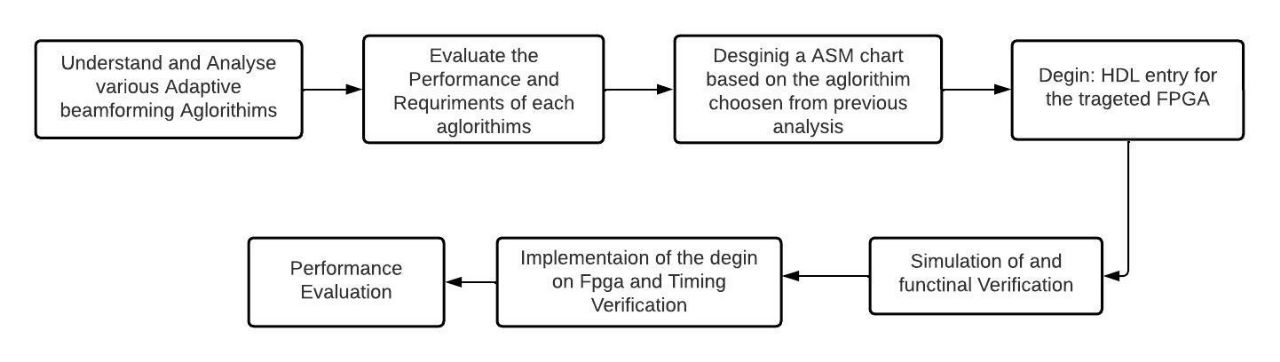
\includegraphics[scale=0.5]{Chapter1/Figures/methodology}	
	\caption{Flow of Work}
	\label{fig:era}
\end{figure}

\section[Assumptions made / Constraints of the project]{\textbf{Assumptions made / Constraints of the project}}
The following assumptions are made while carrying out the work:

\begin{enumerate}
\item Information about grouping of antenna elements into sub array which can be regular or irregular \item Presence of a digital signal processor is assumed which is used as a communication interface between the targeted hardware and the antenna system
\item The implememted algorithm is designed to work with all sizes of inputs and its capability is limited only by the targeted hardware specifications such as the number of LUTs in the FPGA (minimum 3,00,000)
\end{enumerate}

\section[Organization of the report]{\textbf{Organization of the report}}

This report is organized as follows:

\begin{itemize}
\item Chapter 2 discusses the fundamentals of array processing, needs and types of beamforming and the signal models
\item Chapter 3 discusses about the types of algorithms which are suitable for the design of adaptive beamforming and their comparison.   
\item Chapter 4 briefly describes the methodology of the desgin and implementation of the SMI algorithm in Vivado software and optimization technique used to achieve the final design
\item Chapter 5 illustrates the results of the implementated design and comments on the performance of the desgin
\item Chapter 6 tells about the improvisation(s) that can be done and the future scope of the current design
\end{itemize}

.

%Chapter 2
\chapter{Theory and Fundamentals of Array Processing and Beamfoming}

 A technique known as array processing is used to extract information from signals gathered by an array of sensors or antennas.This project aims to showcase a widely used technique for spatial filtering called beamforming, which uses an array of sensors to extract the desired signal that is spatially propagating from a specific direction and identify the strong interferences regions to generate low power and efficient  beam pattern.

\section{ Array fundamentals}

A spatially propagating signal may contain information about both its originating location and the material it is carrying. There are always undesired signals present in addition to the signal, such as noise and intentional and inadvertent interferences. A
single sensor can be used to separate the received signal into its multiple components as long as it has the ability to spatially discriminate the signals based on direction (at the very least). Directivity refers to a sensor’s capacity to spatially distinguish between different signal components received.\textbf{S. haykin} This ability depends on  the geometric structure’s shape and physical properties. Such a single-sensor system, however, has a number of shortcomings. The following are some drawbacks of single sensor/receiver elements:
\begin{itemize}
\item A receiver system based on a single receiver element, similar to a paraboloid dish element, produces a highly directed, high gain sensor with a particular radiation pattern. Every time the reception direction changes, the dish must be mechanically rotated to that precise location in the new direction.
\item The dwell time associated with mechanical rotation is noticeably long, which poses a significant challenge in an adaptive context where the signal circumstances are constantly changing.
\item A single sensor can only be appropriately positioned to receive signals from one direction if it is instantly focused at it; it cannot estimate the DOA of a signal. 
\end{itemize}
The Figure\ref{fig:idea} depicts the beam pattern formed by using an array of sensors that can address these single-sensor limitations, making it suited for many application constraints that single-sensor systems impose on receiver operability.
\begin{figure}[h]
\centering
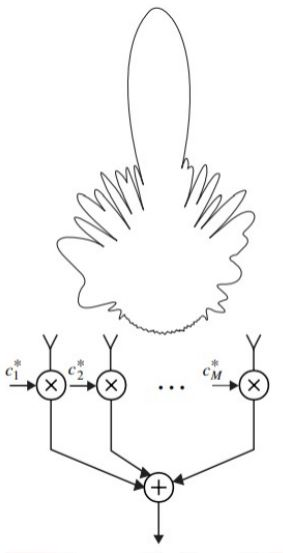
\includegraphics[scale=1]{Chapter2/Figures/idea}		
\caption{ \label{fig:idea}Beam Pattern}
\end{figure}

The sensor array's signals are combined so that one direction is highlighted while others are suppressed or not. The most significant advantage of arrays is that their focus or point can be directed in almost any direction, regardless of how they are arranged. The sensors can be connected in a variety of distinct ways to emphasize different orientations, each of which may carry a Signal of Interest (SoI). Because the various weighted summations of the sensors simply amount to processing the same data in different ways, these many sources can be received at the same time. Arrays can also change the total rejection level in specific directions to counteract a strong interference source.

\section{ Array Model}
The way the array of sensors spatially arranged have  a significant impact on the final beam pattern,which is a crucial factor in determining the array's directivity and performance.Array spacing determines the constructive and destructive interference patterns of the signals received or transmitted by the individual antennas. In this section, we will delve into the effects of different array spacing configurations on the resulting beam pattern, beam-width, side lobes, nulls, and overall directivity of the antenna array. Smaller spacing allows for a finer angular resolution, enabling more precise beam steering. On the other hand, wider spacing may limit the array's ability to steer the main lobe accurately.So the relationship between array geometry and beam pattern is essential for optimizing the array's performance for specific applications.
Various array geometries are commonly used in antenna arrays, each with unique characteristics.
\begin{itemize}
\item Uniform Linear Array (ULA): A linear arrangement of antennas with equal spacing between adjacent elements.Characteristics of the ULA beam pattern, including the main lobe width, side lobes, and nulls.
\item Uniform Rectangular Array (URA):An array with antennas arranged in a rectangular grid, with equal spacing in both the horizontal and vertical directions.
\item Uniform Circular Array (UCA):Antennas arranged in a circular pattern with equal spacing between antennas.Understanding the unique properties of the UCA beam pattern, including azimuthal symmetry.
\item Non-Uniform Array (NRA):An array with antennas placed irregularly, allowing for additional degrees of freedom in beam shaping.
\end{itemize}

\begin{figure}[h]
\centering
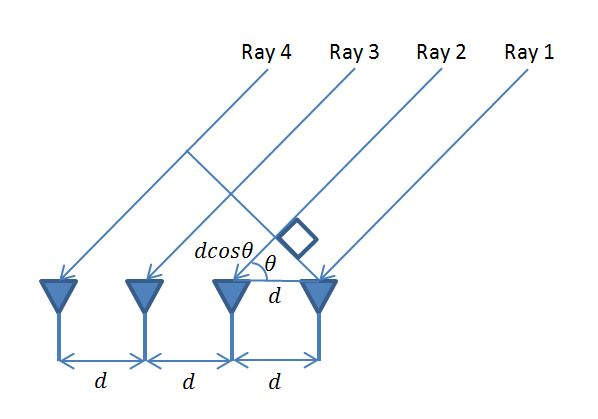
\includegraphics[scale=0.75]{Chapter2/Figures/array}		
\caption{ \label{fig:array}Array of sensors separated distance "d"}
\end{figure}
Figure\ref{fig:array} is an uniform linear array. Consider a single signal that is propagating and strikes the ULA at an angle $\phi$. Due to the fact that all of the elements are similarly spaced, the spatial signal has a difference in propagation pathways between any two sequential sensors of d sin($\phi$), resulting in a temporal delay.This separation and arrangement of  this array elements shows a significant impact on the final beam pattern analysed.
 
\section{Beamforming}
Beamforming is an advanced signal processing technique that is widely used in applications involving antenna or sensor arrays. It enables the manipulation and control of the array's radiation or reception pattern, resulting in better directional sensitivity and signal detection and estimation.Instead of uniformly radiating or receiving signals in all directions, beam forming concentrates the energy of the array in a specific direction while decreasing receptivity to signals from other directions. This capacity to selectively direct the array's beam provides considerable benefits in terms of enhanced SNR, interference rejection, and spatial selectivity.\\
The fundamental idea of beamforming is to modify the phase and amplitude of signals received or transmitted by individual array elements. By adjusting the phases and amplitudes of the signals, constructive interference occurs in the desired direction, amplifying the signal, while destructive interference occurs in other directions, reducing undesirable signals. This causes the array's emission or reception pattern to form a narrow and focussed main lobe, which can be electronically guided to track a target or optimize reception.\\
\subsection{Non Adaptive beamforming}
   Non-adaptive beamforming is a traditional beamforming technique used in antenna arrays and sensor arrays to create a fixed, predetermined beam pattern.Non-adaptive beamforming relies on carefully designing and setting the array's weights or coefficients to achieve a specific desired beam pattern. These weights are determined during the design phase and remain constant during signal processing. By controlling the phase and amplitude of the signals transmitted or received by each element in the array, non-adaptive beamforming creates a narrow main lobe in the desired direction, providing enhanced sensitivity to signals from that direction.This fixed beam pattern is particularly useful in applications where the array needs to maintain a steady direction of focus, such as in radar systems for tracking specific targets or in wireless communication systems for coverage in a specific direction.This are simple,easy and cost less to design but they lack adaptability which is essential for the modern applications.
\subsection{Adaptive beamforming}   
   Adaptive beamforming is a smart signal processing technique used in antenna arrays and sensor arrays to dynamically alter the weights or coefficients of the array based on the received data. 
This is achieved by iteratively updating the weights in response to the received signals. Adaptive algorithms use statistical properties of the received signals to estimate the optimal set of weights that maximize the array's directivity towards the desired signal while minimizing sensitivity to interference and noise.As the signal environment evolves, the array adapts its beam direction to track moving targets or to null out interference sources, resulting in enhanced performance and improved signal-to-interference-plus-noise ratio (SINR).
\begin{figure}[h]
\centering
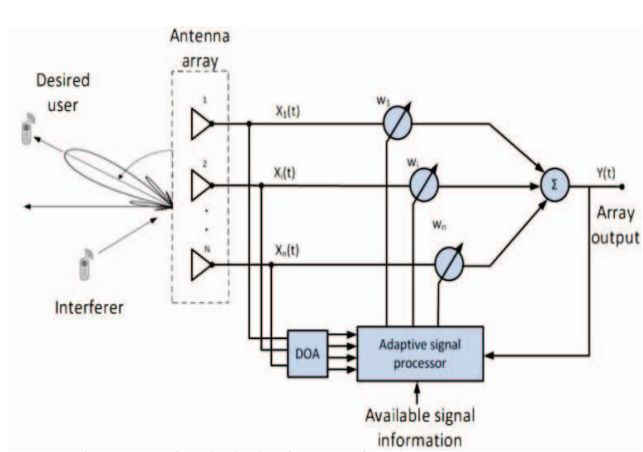
\includegraphics[scale=0.75]{Chapter2/Figures/1}		
\caption{ \label{fig:1}Adaptive Beamformer Design}
\end{figure} 

\section{Need of subarrays in Adaptive Beamforming}
 As discussed in the above sections when we use a array of sensors as a transmitter or a receiver we need to deal with a delay to achieve required beam pattern.In fixed beamformer its done by physically adjusting antenna elements and in adaptive beamformer an electronic unit(time delay units) adjusts this delays.So this electronic units makes adaptive beamforming algorithms can be computationally intensive, especially when applied to large-scale antenna arrays.To avoid this we can using simple phase shifter but they work efficiently fixed range of frequencies and introduces beam squints in the presences of other frequencies.So as a tradeoff we use both phase shifters and time units by using the concept of subarrays.\\
\begin{figure}[h]
\centering
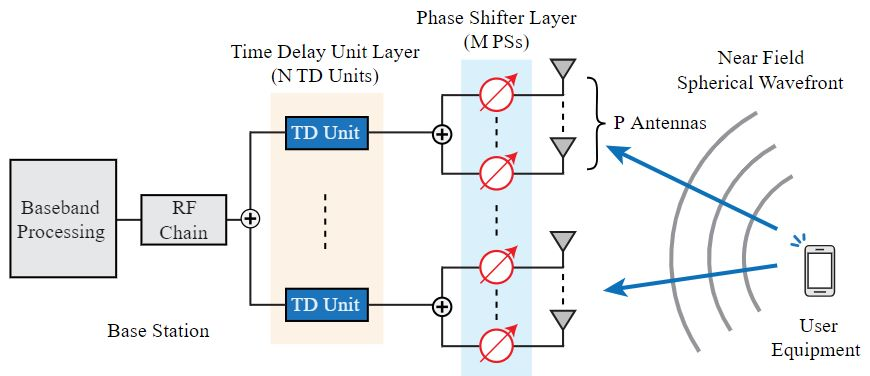
\includegraphics[scale=0.8]{Chapter2/Figures/1 main}		
\caption{ \label{fig:1}Adaptive beamforming using subarrays}
\end{figure} 

Subarrays provide additional degrees of freedom in beamforming design. By configuring multiple subarrays with varying positions, orientations, or element spacings, adaptive beamforming gains greater flexibility in shaping the beam pattern. This enhances the array's ability to track multiple targets simultaneously, adjust to non-stationary signals, and optimize performance for specific signal scenarios.\\
Subarrays are particularly useful in achieving adaptive nulling, where unwanted interference or jamming signals are suppressed. By configuring subarrays with spatial separation, adaptive algorithms can steer nulls toward interference sources while maintaining sensitivity to the desired signals. This results in improved interference rejection and a higher signal-to-interference-plus-noise ratio (SINR)  
 
\section{Use of Acronyms and Glossaries}
Acronyms are nothing but the short form of regular repeated word. Say for example, you have a repeat word "Integrated Circuits" and you want to use a short form for it as "IC". For which you have to first define the word and use it wherever you wanted to refer it.

First, let's look at the definition, which has to be entered in \texttt{Glossaries.tex} under \texttt{CoverPages} directory.
\begin{verbatim}
%\newacronym{<Ref>}{<Short-Form>}{<Expanded word>}
\newacronym{ic}{IC}{Integrated Circuits}
\end{verbatim}
In order to use the defined acronym, use the commands \verb|\gls{<Ref>}| as shown below

As an example, call the definition with \verb|\gls{ic}| and the outcome of it is reflected as, \gls{ic}.

Note: For the First time, the expanded form appears along with the Short-form definition inside parenthesis. But when the \verb|\gls{}| is repeated, only Short-form appears inside the parenthesis.

Now, let's look at the definition of symbols. Follow the syntax to define the symbol first, inside \texttt{Glossaries.tex} under \texttt{CoverPages} directory.
\begin{verbatim}
%\newglossaryentry{<Ref>}{name=<Symbol>, description={<description about the symbol>}, type=<List type>}
\newglossaryentry{rc}{name=$\tau$, description={Time constant}, type=symbolList}
\end{verbatim}

As an example, the rate of change is defined with \verb|\gls{rc}| and the outcome of it is reflected as, the rate of change is defined with \gls{rc}.

\vspace{0.75cm}

 \textbf{The chapters should not end with figures, instead bring the paragraph explaining about the figure at the end followed by a summary paragraph.}

After elaborating the various sections of the chapter (From Chapter 2 onwards), a summary paragraph should be written discussing the highlights of that particular chapter. This summary paragraph should not be numbered separately. This paragraph should connect the present chapter to the next chapter.

%Chapter 3
\chapter{Techniques for Adaptive Beamforming}

\indent\indent Here, we discuss three algorithms used for adaptive beamforming. Advantages, disadvantages and a a brief about each algorithm is provided. The final output that is of weight updation is correlated with the beamforming techniques considered. The main considerations include the input signal sample consideration, obtaining minimum variance, minimum Interference to Noise Ratio (INR) (SNR maximisation). Under these conditions, the two main categories considered are the sample by sample based adaptive
techniques and the block adaptive based techniques. Beamformer under these are studied,
implemented and compared under the same signal, noise and interference conditions.

\section{Sample by sample techniques}

The optimal beamformer can be found by techniques that compute the beamforming weights sample by sample and update the weights for each new sample. Over here, least squares problem is solved in a constrained way rather than an unconstrained one which differentiates it from adaptive filters. As a result, we have the steering vector, in contrast to the cross-correlation vector,thus is a priori and is not derived from the data. The main techniques explored under this include least mean square technique and recursive least mean square.

\subsection{Least mean squares}
This type of estimation, minimizes the sum of squares of the estimated error, requires the measurement of both the input signal and the desired response signal. A set of measurements of the desired response y(n) and the input signals xk(n) for k from 1 to M has been taken for n from 0 to N - 1. The task is to estimate the desired response y(n) using the linear combination given as in \ref{eq:1}

\begin{equation} \label{eq:1}
\hat(y)(n) = \sum_{k=1}^{M} c_{k}^{*}x(n) = c^{H}(n)x(n)
\end{equation}

where estimation error is defined as in \ref{eq:2}

\begin{equation} \label{eq:2}
e(n) = y(n) - \hat(y)(n) = y(n) - c^{H}(n)x(n)
\end{equation}

The coefficients of the combiner are hence computed by minimizing the sum of the
squared errors is described as in \ref{eq:3}

\begin{equation} \label{eq:3}
E = \sum_{n=0}^{N-1} |e(n)|^{2}
\end{equation}


\subsection{Recursive least squares}
This technique also revolves about a constrained rather than an unconstrained optimization. Here, y(n) as discussed in the previous section is not the desired response. However, for the adaptive beamformer the steering vector is used, which is deterministic. Algorithms based on RLS methods can be implemented such that the output y(n) is computed directly (direct output extraction) or the adaptive beamformer weights are computed and then applied to determine the output. The RLS methods are based on the update equation of the estimate of the correlation matrix is given as described in \ref{eq:4}

\begin{equation} \label{eq:4}
\hat(R_{x})(n+1) = (\Lambda)_{rls}\hat(R_{x})(n) + x(n+1)x^{H}(n+1)
\end{equation}


where $0 < \lambda_{rls} \le 1$ is a scalar sometimes referred to as the forgetting factor.\vspace{0.75cm}

\section{Block adaptive techniques}
In this techniques, a block of data is used to determine the beamformer weight vectors. The sample matrix inversion fall under this category of technique. The estimates of the statistics used by these methods are based on the data, but they are updated with each block of samples.

\subsection{Sample matrix inversion}
In the real-time context, correlations must be deduced from the incoming data. The ML estimate of the correlation matrix is therefore given by the average of the outer products of the array snapshots: where the indices nk define the K samples of $x_{i} + n(n)$ for 1 n N that make up the training set. The obtained ML estimate of the correlation matrix implies that as K $\rightarrow \infty$, then $R_{i}+n \rightarrow R_{i}+n$. The number K of snapshots utilised to compute the sample correlation matrix is the sample support. The estimate improves with increasing sample size $R_{i+n}$ of the correlation matrix for stationary data. Substituting the sample correlation matrix into the optimum beamformer weight computation as given in \ref{eq:5}

\begin{equation} \label{eq:5}
c_{smi} = \dfrac{\hat(R)_{i+n}^{-1}v(\phi_{S}}{v^{H}(\phi_{s}\hat(R)_{i+n}^{-1}}
\end{equation}


The resulting beampattern obtained from this procedure is defined as the SMI based beamformer.

\section{Choosing adaptive beamforming algortithm}
The electronic scanning unit takes available info (from DOA), feedback from output and generates certain information array factors or weights which adjusts the time delay units and phase shifters to produce desired beam pattern. To compute this weights we require  adaptive beamforming algorithms such as Least mean square(LMS), Recursive Least Square(RLS) or To compute this weights we require  adaptive beamforming algorithms such as Least mean square(LMS), Single Matrix Inversion(SMI) or Recursive Least Square(RLS) as discussed above.

\begin{itemize}
\item LMS is an iterative process which corrects its output by considering the error from previous data but to converge it requires many iterations.
\item SMI  converges faster than LMS as it uses inverse of correlation matrix. But it is computationally complex.
\item RLS encompasses features of both SMI and LMS as it converges faster but has higher margin of error than SMI but lesser than LMS.
\end{itemize}
The targeted hardware that is the FPGA is capable of handling computationally expensive operations and hence, we choose SMI for the implementation of the adaptive beamforming algorithm to get optimal beamformer weights.

\section{MATLAB design for weight calculation}
Regular subarrays are used as antenna elements. Required Frequency, wavelength, spacing between the antenna elements are taken as the design parameters. Signal required to be detected is generated and the jammers as interference signals by using SNR, azimuth angle, elevation angle. Taking the above signals as inputs to the standard SMI Algorithm, optimal beamformer weights are are calculated. It is to be noted that the subarray matrix is using an existing algorithms that leads to a better adaptive beamforming design.

\begin{figure}[H]
\centering
	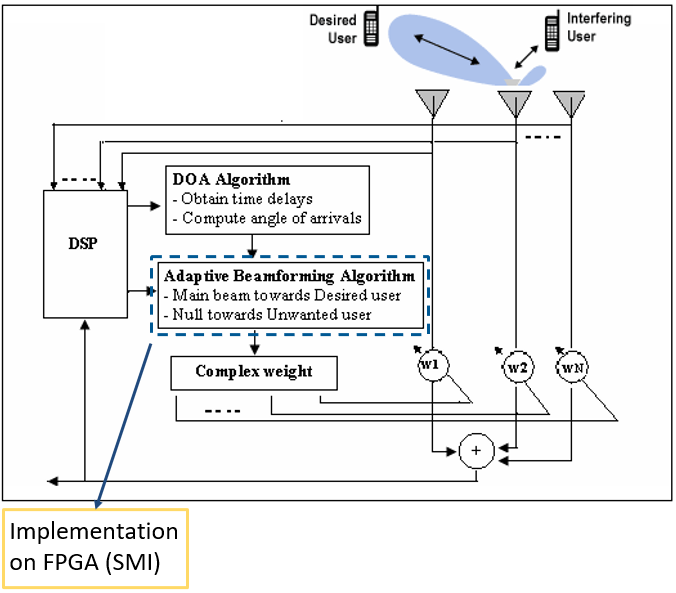
\includegraphics[scale=0.7]{Chapter3/Figures/matlab_algo}	
	\caption{\label{fig:matlab_algo}SMI Algorithm implemented at position shown}
\end{figure}

%Chapter 4
\chapter{Implementation of Pipelined Analog to Digital converter}

\indent\indent From Chapter 2 onwards, every chapter should start with an introduction paragraph. This paragraph should brief about the flow of the chapter. This introduction can be limited within 4 to 5 sentences. The chapter heading should be appropriately modified (a sample heading is shown for this chapter).But don't start the introduction paragraph in the chapters 2 to end with "This chapter deals with....". Instead you should bring in the highlights of the chapter in the introduction paragraph. 

\section{Contents of this chapter}
This chapter should elaborate the following in detail.
\begin{enumerate}
\item Implementation details for hardware based projects
\item Top level Design for software based projects
\end{enumerate}

You can add sections and sub sections to elaborate your project work done.

\vspace{0.75cm}

 \textbf{The chapters should not end with figures, instead bring the paragraph explaining about the figure at the end followed by a summary paragraph.}

After elaborating the various sections of the chapter (From Chapter 2 onwards), a summary paragraph should be written discussing the highlights of that particular chapter. This summary paragraph should not be numbered separately. This paragraph should connect the present chapter to the next chapter. 



%Chapter 5
\chapter{Results \& Discussions}
\indent\indent From Chapter 2 onwards, every chapter should start with an introduction paragraph. This paragraph should brief about the flow of the chapter. This introduction can be limited within 4 to 5 sentences. The chapter heading should be appropriately modified (a sample heading is shown for this chapter).But don't start the introduction paragraph in the chapters 2 to end with "This chapter deals with....". Instead you should bring in the highlights of the chapter in the introduction paragraph.
\section{Contents of this chapter}
All the results obtained for your objectives should be discussed in this chapter. This chapter should contain the following sections as per the project.
\begin{enumerate}
\item Simulation results
\item Experimental results
\item Performance Comparison
\item Inferences drawn from the results obtained
\end{enumerate}
All the figures should be properly explained by bringing the scenarios of the design done in the project. A detailed discussion of results obtained should be done in this chapter.

\section{Tables in thesis}
\begin{itemize}
	\item All Table Caption should be in Sentence Case, TNR 10 Pt. It should be of the Format:
	\begin{itemize}
		\item Table 1.1 Results of the experiment ….(Centered)
	\end{itemize}
	\item It should be cited as Table 1.1.
	\item Caption should appear above the Table.
	\item Table Header and the entries should be of Font TNR 10 Pt, Justified.
	\item For wider Table, the page orientation can be Landscape.
	\item For Larger Table, it can run to pages and the header should be repeated for each page of the Table.
	\item Table must be adjusted to fit in the page and no single row is left out for a new page.	
\end{itemize}

Sample Table \ref{c5:tab1} is given below for your reference,

\begin{table}[htb]
\fontsize{10}{12}\selectfont
\caption{Country List}
\label{c5:tab1}
\begin{tabular}{|p{3cm}|c|c|c|}
	%\hline
	%\multicolumn{4}{|c|}{Country List} \\
	\hline
	\textbf{Country Name     or Area Name}& \textbf {ISO ALPHA 2 Code} & \textbf {ISO ALPHA 3 Code} & \textbf{ISO numeric Code}\\
	\hline
	\textbf{Afghanistan}   & AF    & AFG &   004\\\hline
	\textbf{Aland Islands}&   AX  & ALA   & 248\\\hline
	\textbf{Albania} & AL & ALB&  008\\\hline
	\textbf{Algeria}    &DZ & DZA&  012\\\hline
	\textbf{American Samoa}&   AS  & ASM&016\\\hline
	\textbf{Andorra}& AD  & AND   & 020\\\hline
	\textbf{Angola}& AO  & AGO& 024\\
	\hline
\end{tabular}
\end{table}

%\begin{table}[htp]
%\fontsize{10}{12}\selectfont
%\centering
%\caption{Data units, sources, and dates} \label{c5:tab2}
%\begin{tabular}{| *4{>{\arraybackslash}m{1in}|} @{}m{0pt}@{}}
%	\hline
%	\textbf{Variable} & \textbf{Dates} & \textbf{Units} &
%	\textbf{Source}  &\\[2ex] 
%	\hline
%	\textbf{Nominal Physical Capital Stock} & 1950-1990 & Billions
%			US\$ & Nehru and Dhareshwar (1993) &\\[0ex]
%	\hline
%	\textbf{Total Population} & 1950-1990 & Billions & Nehru and
%			Dhareshwar (1993) &\\[0ex]
%	\hline
%	\textbf{Nominal GDP} & 1950-1990 & Billions  US\$ & PWT &\\[5ex]
%	\hline
%	\textbf{Real GDP per capita} & 1950-1990 & 2005 US\$ per capita & PWT &\\[5ex]
%	\hline
%\end{tabular}
%\end{table}

\section{Math equation in thesis}
All equation should be written using equation editor or using an equivalent tool.
\begin{itemize}
	\item Equations should be numbered as : 1.1, 1.2 ...
	\item Equation should be Centered, 12 Pt, TNR. 
	\item Equation number should be right Justified
	\item It should be cited as Eqn. 1.1.
   \item If the sentence starts by citing an equation, then it should be written as Equation 1.1 For example, Equation 5.1 states the Pythagoras theorem.

	
\end{itemize}

For example in Eqn. \ref{c5:eqn1}, The well known Pythagorean theorem $x^2 + y^2 = z^2$ was 
proved to be invalid for other exponents. 
Meaning the next equation has no integer solutions:

\begin{equation}
\label{c5:eqn1}
	x^n + y^n = z^n
\end{equation}

The mass-energy equivalence is described by the famous equation in Eqn. \ref{c5:eqn2}
\begin{equation}
\label{c5:eqn2}
	E=mc^2
\end{equation}

discovered in 1905 by Albert Einstein. 

\vspace{0.75cm}

 \textbf{The chapters should not end with figures, instead bring the paragraph explaining about the figure at the end followed by a summary paragraph.}

After elaborating the various sections of the chapter (From Chapter 2 onwards), a summary paragraph should be written discussing the highlights of that particular chapter. This summary paragraph should not be numbered separately. This paragraph should connect the present chapter to the next chapter.





%Chapter 6
\chapter{Conclusion and Future Scope}

\section{Conclusion}
This chapter should not contain an introduction paragraph like other chapters. You can directly write conclusion of the work done under this section. Typically this section can have 3 to 4 paragraphs. 

First paragraph should bring in the scenario of the project and every objective should be explained here.

Second paragraph should say how the objectives are implemented and achieved.

Last paragraph should draw the conclusions from each objective with quantitative results, performance improvement etc. 

\section{Future Scope}
Briefly discuss the constraints and limitations of the project and state the possibilities of extending the work in future.
\section{Learning Outcomes of the Project}
\begin{itemize}
\item List the learning outcomes here
\item List a minimum of 5 learning outcomes
\end{itemize}



%% Uncomment the following 2 commands to add Appendix chapters
\appendix
\chapter{Code}
\section{First Appendix}
You can use \texttt{tcblisting} for creating the code snippets. The following example illustrates how one can customize the \texttt{tcblisting} to achieve the \texttt{tcl} script. Similarly, one can use it for other programming language listing, including HDL.

\begin{tcblisting}{listing only,colback=gray!10!white, breakable, boxsep=0pt,top=1mm,bottom=1mm,left=1mm,right=1mm,
listing options={
language= tcl,
basicstyle=\small\ttfamily, 
otherkeywords={create_clock, set_clock_latency, set_input_delay, set_output_delay, set_load, set_max_fanout, set_fanout_load},
keywordstyle=\color{blue}, 
%keywordstyle=[2]{\color{red}},
commentstyle=\color{gray},
backgroundcolor=\color{gray!25},
%morekeywords=[2]{arg,pos},
%moredelim=[is][\color{violet}]{''}{''},
escapechar=!}}
# Since our design has a clock with name clk, 
## specify that name under [get_port ]
create_clock -period 40 -waveform {0 20} [get_ports clk]

# Setting a 'delay' on the clock:
set_clock_latency 0.3 clk

# Setting up constraints on your I/P and O/P pins
set_input_delay 2.0 -clock clk [all_inputs]!\tikz[remember picture]\node[](c1){};!
set_output_delay 1.65 -clock clk [all_outputs]!\tikz[remember picture]\node[](c2){};!

# Set realistic 'loads' on each output pin
set_load 0.1 [all_outputs]

# Set 'maximum' fanin and fan-out for the input and output pins 
set_max_fanout 1 [all_inputs]
set_fanout_load 8 [all_outputs]      
\end{tcblisting}
%Appendix Chapter 1

\backmatter
\clearpage
\printbibliography%

\end{spacing}
\end{document}